%************************************************
\chapter{Clustering and Classification using Topics}\label{ch:clustering-and-classification}
%************************************************

% \renewcommand\thefigure{\arabic{figure}}
% \setcounter{figure}{1}

\setcounter{con}{0}

The various experiments in the preceding chapters culminated in demonstrating that topics can be used to tell apart fake from authentic news texts. This can be achieved using the unique representation of topics from the opening and remainder sections of news articles. This conclusion was arrived at following statistical tests, which showed that there is some evidence that fake and real news may differ thematically.

In this study, the utility of topic representations using simple methods is analysed. First, through unsupervised learning, clustering; and second, through supervised learning, classification. The most straightforward possible \ac{ML} methods are selected here because the goal is to evaluate the utility of these representations. It should be noted that the topic distributions themselves are used as features in this case, rather than the divergence scores calculated from them. Therefore, the experiments in this chapter are not based on the calculated variance between topics in the opening and remainder parts of fake and real articles per se. Nonetheless, this information is still retained in the distributions.

As related in \autoref{ch:related-work}, both approaches (\emph{i.e.}, clustering and classification) have been used by several works in the literature on misinformation detection. Their advantages and shortcomings, particularly in the context of misinformation, are also discussed therein.

Clustering is done using the $K$-means algorithm. Having performed feature extraction in an unsupervised way, it is additionally beneficial to further detect misinformation likewise. A wide range of classifiers was experimented with, including Decision Trees, Random Forest and \ac{SVM}.

\section{Clustering}
\label{sec:5-clustering}

This experiment was carried out on whole topic distributions from the opening and remainder sections of articles, as well as their reduced 2D vectors (called the \emph{Aggregate} method here).

\paragraph{Problem definition:}The $K$-means algorithm requires us to specify the number of clusters outputted, $K$.
 The evaluation for this experiment, detailed later in this subsection, will focus on determining whether the clusters are becoming \emph{pure} or not.

\paragraph{Datasets and data:}The datasets used in this experiment are the same as in \autoref{ch:thematic-coherence}\sidenote{See \sectionref{ssec:4-datasets}.} except for GMI because it was only considered as a first step in the other experiments. The same topic data was used too, except that it is shortened here, which is to say, $N = \{ 10, 20, 30, 40, 50 \}$.\sidenote{See Algorithm \autoref{4-divergence} in \sectionref{ssec:4-LDA}.} Therefore, there is a $(1 \times 150)$ topic distribution for each article.

\paragraph{Conjectures and baselines:}Three baselines were formulated to assess and compare the utility (based on the clustering metric used hereinafter) of extracting topic features from articles in different ways. For example, whether using reduced dimensions of the topic features improve the clustering. Or, if extracting features from two sections of an article is any better than taking topics from the entire text.

\begin{con}
  \label{con:a}\textit{Topics extracted from the opening and remainder sections of articles improve clustering (Aggregate method), compared with topics extracted from the whole document.}
\end{con}

\emph{Baseline 1} was created to evaluate \Cref{con:a}. Here, topics (10, 20, 30, 40, and 50) are extracted from entire documents, instead of from their openings and remainders. Therefore, each document is represented as a single 150-dimensional vector. $K$-means (with $K = 2$ and the maximum number of iterations set to 500) is run on the original 150D topic distribution, as well as on their reduced dimension (2D) vectors. The projection-based dimensionality reduction methods experimented with are: Autoencoder, \ac{tSNE}, and \ac{UMAP}. The component-based methods used are: Linear, \ac{NMF}, \ac{PCA}, and \ac{SVD}.

\begin{con}
  \label{con:b}\textit{Combining multiple topic distributions also improves clustering, compared with individual topics on their own.}
\end{con}

\emph{Baseline 2} tests \Cref{con:b}: individual topic distributions (for 10, 20, 50, and 100 topics) from the opening and remainder sections form the clustering data. For example, the vector for 10 topics will be a $(1 \times 20)$ vector.

\begin{con}
  \label{con:c}\textit{Clustering performs better than simply assigning examples to classes randomly.}
\end{con}

\emph{Baseline 3} tests \Cref{con:c}: here, the quality of clustering is calculated based on random assignment to each class, \emph{i.e.}, half of each type of news forms a cluster.


\paragraph{Evaluation:} There are two main ways to evaluate the quality of clustering: \emph{internal} and \emph{external} criteria.\sidecite{Manning:2008} Ideally, articles within a given cluster should be similar (inter-cluster similarity), and those from different clusters should be dissimilar (intra-cluster similarity). This is the basis of the internal criterion. On the other hand, the external criterion requires a benchmark created by people who can expertly categorise each item. As it takes account of the nuances of a given application, the external criterion is more reliable, especially if a model is to be deployed in the real world. It is applicable in this case since the data is fully labelled. One such criterion, \emph{Purity}, was used in this experiment to evaluate the aforementioned baselines. Following \citeauthoryear{Manning:2008}, it can be defined as:

\begin{equation} \label{eq:5-purity}
purity\left( \Omega, C \right) = \frac{1}{D} \sum _{k = 1}^K \: \underset{j = 1 \ldots J}{\max} \: \left| \omega_k \cap c_j \right|
\end{equation}
\begin{conditions}
 \Omega    &  $\{ \omega_1, \omega_2, \ldots, \omega_K \}$ is a set of clusters \\
 C         &  $\{ c_1, c_2, \ldots, c_J \}$ is a set of classes \\
 D         &  total number of documents \\
 \omega_k  &  set of documents in \omega_k \\
 c_j       &  set of documents in c_j
\end{conditions}

The most frequent class of articles--fake or real--in a cluster is assigned as the label of that cluster. Therefore, the accuracy of the clustering is the sum of fractions of correct assignments in each cluster. This summarises purity as a metric.

\autoref{fig:5-2D-plot} shows plots of the concatenated 300D data, with their dimensions reduced to 2D, using the \emph{Linear} method for dimensionality reduction in Wolfram Mathemematica.\sidecite{Wolfram:2021b} Each data point is coloured according to its class. It can be observed from the figure that reducing the dimensions removes superfluous information while preserving the essential information that apparently differentiates the two types of news. Significant variations can be observed in the topic distributions of fake and real news in all datasets, except for BuzzFeed.

Put simply, when it comes to both fake and real articles talking about the same subject, even across various domains, there are noticeable variations in how they approach the topic in the beginning and the rest of the articles. This observation is in agreement with the outcomes of previous experiments, that topics are an effective feature for detecting misinformation. Naturally, the boundaries between the clusters are not clear-cut. For example, there is a discernible overlap among the clusters in the ISOT dataset, indicating the presence of both counterfeit and genuine articles that nsimilarly narrate stories. However, notable differences can be seen when examining multiple fabricated and legitimate articles in general.

\begin{figure}[htp]
    \centering

    \subfloat[\centering ]{
    \begin{minipage}{240pt}{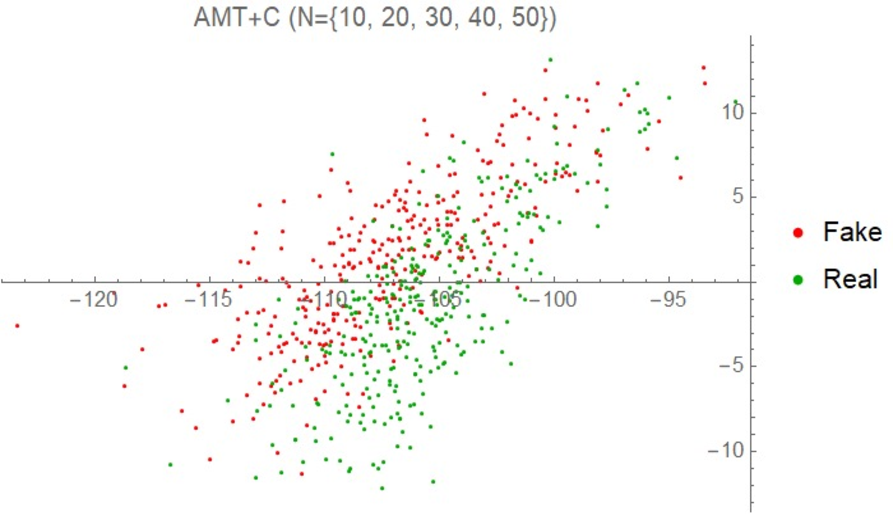
\includegraphics[width=230pt]{gfx/5_2d_clustering_amt+c} }
    \end{minipage}
    }
    \subfloat[\centering ]{
    \begin{minipage}{240pt}{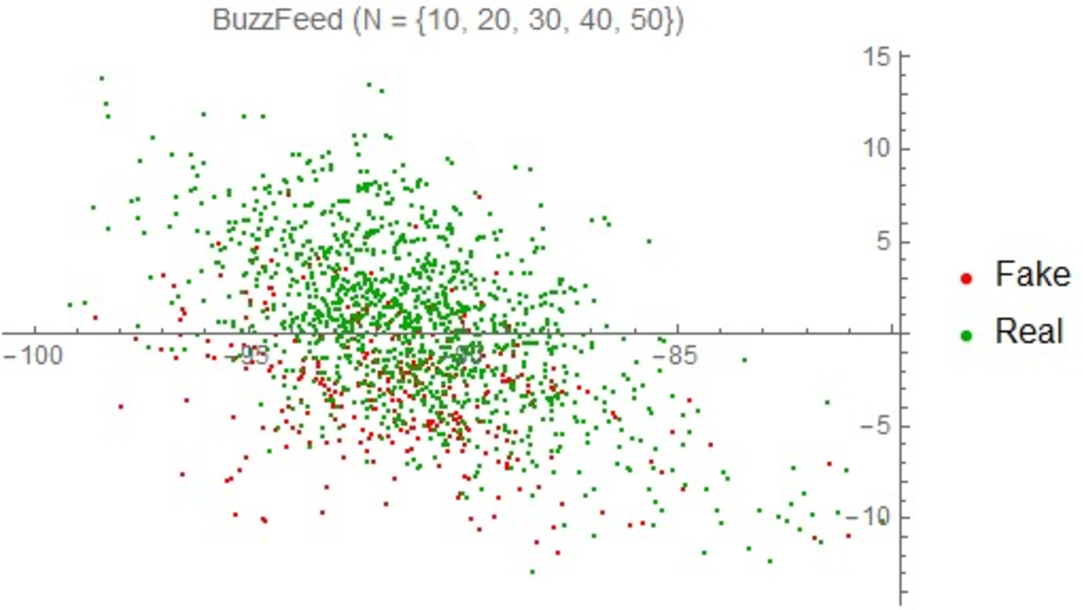
\includegraphics[width=230pt]{gfx/5_2d_clustering_bf} }
    \end{minipage}
    }

    \subfloat[\centering ]{
    \begin{minipage}{240pt}{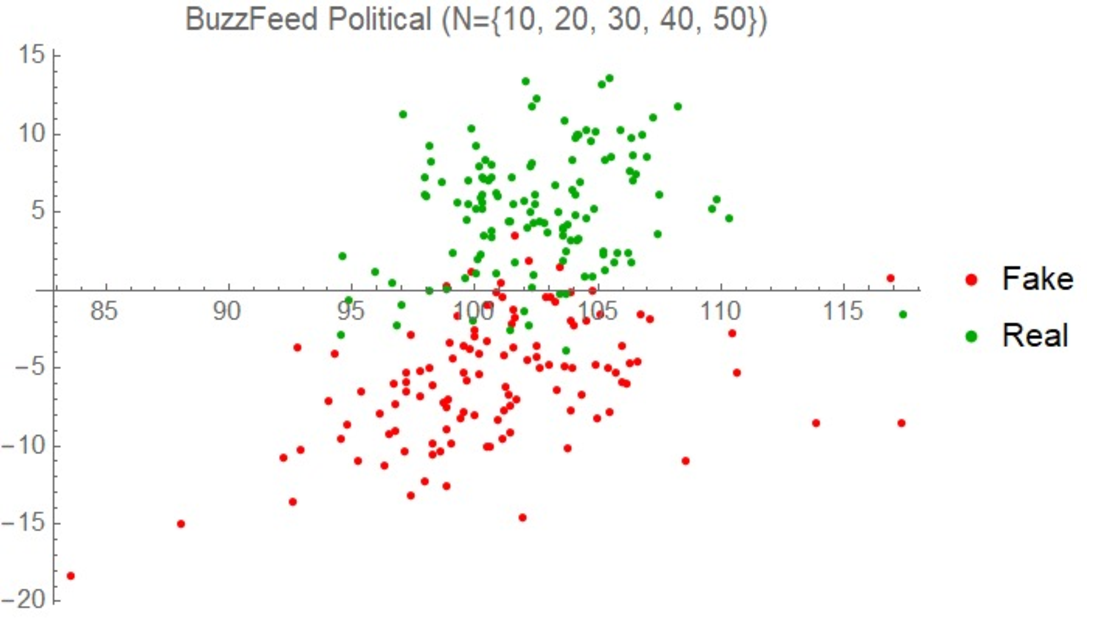
\includegraphics[width=230pt]{gfx/5_2d_clustering_bfp} }
    \end{minipage}
    }
    \subfloat[\centering ]{
    \begin{minipage}{240pt}{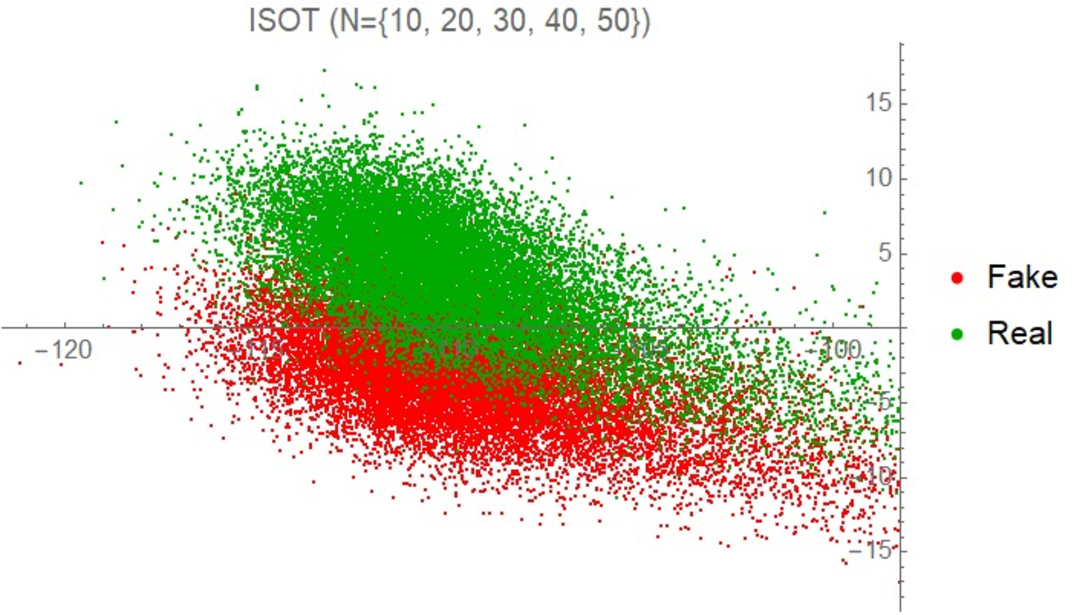
\includegraphics[width=230pt]{gfx/5_2d_clustering_isot} }
    \end{minipage}
    }
\end{figure}

\begin{figure}[htp]
    \ContinuedFloat \centering

    \subfloat[\centering ]{
    \begin{minipage}{240pt}{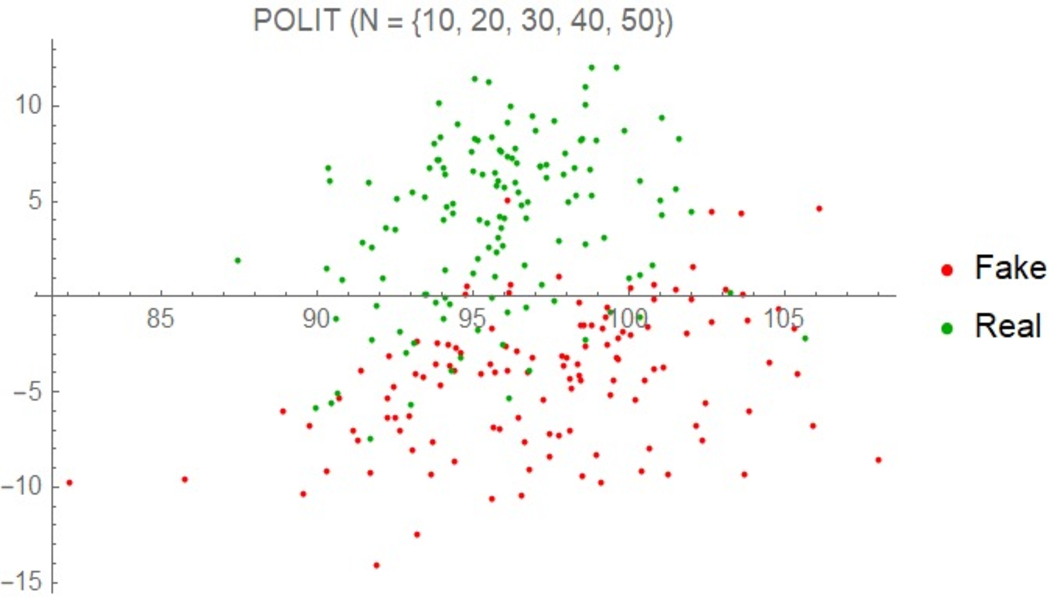
\includegraphics[width=230pt]{gfx/5_2d_clustering_polit} }
    \end{minipage}
    }
    \subfloat[\centering ]{
    \begin{minipage}{240pt}{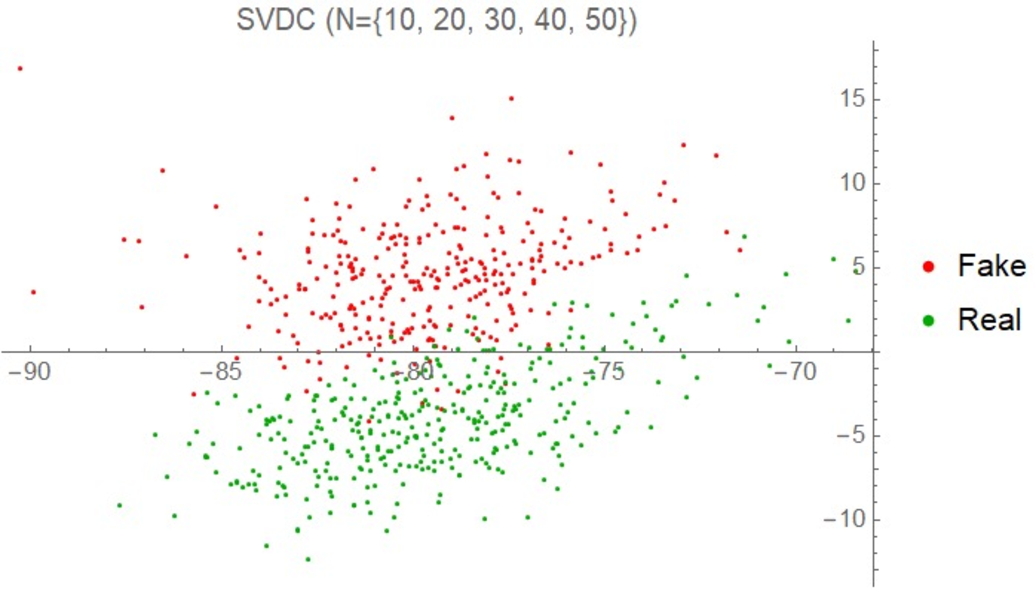
\includegraphics[width=230pt]{gfx/5_2d_clustering_svdc} }
    \end{minipage}
    }

    \centering
    \caption{2D plots of dimension-reduced topic distributions for datasets used.}
    \label{fig:5-2D-plot}
\end{figure}
\FloatBarrier

\paragraph{Results and discussion:} \autoref{tab:5-purity-b1} shows results for the evaluation of Baseline 1 on the different data dimensions experimented with. Two values, 100 and 200, were used for the \ac{tSNE} parameter \emph{perplexity}.\sidenote{Note that this notion of perplexity is different from the one discussed in \autoref{ssec:4-coherence-perplexity}.} For \ac{UMAP}, two values, 50 and 100, were used for the number of neighbours. \autoref{tab:5-purity-b2} shows results for the evaluation of Baseline 2.

\begin{sidewaystable}[htp]
\begin{tabular}{ >{\raggedright}p{2cm} *{12}{c} }
\toprule
\multirow{2}{2cm}{ \tableheadline{Dimension} } & \multicolumn{2}{c}{ \tableheadline{AMT+C} } & \multicolumn{2}{c}{\spacedlowsmallcaps{BuzzFeed}} & \multicolumn{2}{c}{ \tableheadline{\shortstack[l]{BuzzFeed-\smallskip\\Political}} } & \multicolumn{2}{c}{\tableheadline{ISOT}} & \multicolumn{2}{c}{\tableheadline{POLIT}} & \multicolumn{2}{c}{\tableheadline{SVDC}} \\
\cmidrule(lr){2-3} \cmidrule(lr){4-5} \cmidrule(lr){6-7} \cmidrule(lr){8-9} \cmidrule(lr){10-11} \cmidrule(lr){12-13} &
\spacedlowsmallcaps{Agg} & \spacedlowsmallcaps{B1} & \spacedlowsmallcaps{Agg} & \spacedlowsmallcaps{B1} & \spacedlowsmallcaps{Agg} & \spacedlowsmallcaps{B1} & \spacedlowsmallcaps{Agg} & \spacedlowsmallcaps{B1} & \spacedlowsmallcaps{Agg} & \spacedlowsmallcaps{B1} & \spacedlowsmallcaps{Agg} & \spacedlowsmallcaps{B1} \\

\midrule
150D / 300D           & 0.5179 & 0.5367 & 0.7858 & 0.7858 & 0.5205 & 0.5226 & 0.5679 & 0.5346 & 0.6211 & 0.5234 & 0.7169 & 0.5452 \\
Autoencoder           & 0.5179 & 0.5320 & 0.7858 & 0.7858 & 0.5220 & 0.6872 & 0.5453 & 0.5345 & 0.5234 & 0.6523 & 0.6221 & 0.5301 \\
2D, Linear            & 0.5133 & 0.5211 & 0.7858 & 0.7858 & 0.8150 & 0.7078 & 0.5897 & 0.5579 & 0.7031 & 0.6602 & 0.5949 & 0.5301 \\
2D, NMF               & 0.5086 & 0.5226 & 0.7858 & 0.7858 & 0.5410 & 0.5225 & 0.5844 & 0.5409 & 0.5820 & 0.5234 & 0.7334 & 0.5557 \\
2D, PCA               & 0.5195 & 0.5413 & 0.7858 & 0.7858 & 0.6271 & 0.5226 & 0.5346 & 0.5346 & 0.6211 & 0.5234 & 0.7500 & 0.5437 \\
2D, SVD               & 0.5117 & 0.5288 & 0.7858 & 0.7858 & 0.5574 & 0.5226 & 0.5608 & 0.5346 & 0.6094 & 0.5234 & 0.7425 & 0.5422 \\
2D, TSNE [$p=100$]    & 0.5055 & 0.5273 & 0.7858 & 0.7858 & 0.9016 & 0.5226 & 0.5591 & 0.5346 & 0.7648 & 0.5625 & 0.7892 & 0.5723 \\
2D, TSNE [$p=200$]    & 0.5179 & 0.5273 & 0.7858 & 0.7858 & 0.8893 & 0.5597 & 0.5826 & 0.5346 & 0.7617 & 0.5430 & 0.8298 & 0.5723 \\
2D, UMAP [$nn=50$]    & 0.5226 & 0.5445 & 0.7858 & 0.7858 & 0.5205 & 0.5597 & 0.5828 & 0.5346 & 0.5742 & 0.5391 & 0.5301 & 0.5768 \\
2D, UMAP [$nn=100$]   & 0.5304 & 0.5445 & 0.7858 & 0.7858 & 0.5205 & 0.5597 & 0.5815 & 0.5346 & 0.5547 & 0.5391 & 0.6054 & 0.5768 \\
\bottomrule
\end{tabular}
\caption{Purity scores for Baseline 1 (B1) and Aggregate (Agg) methods. $p$ = perplexity, $nn$ = number of neighbours.}
\label{tab:5-purity-b1}
\end{sidewaystable}
\FloatBarrier

\begin{table}[htp]
\addlinespace
    \begin{tabularx}{\textwidth}{Xlll} \toprule
        \tableheadline{Dataset} & \tableheadline{$T = 10$} & \tableheadline{$T = 20$} & \tableheadline{$T = 50$} \\
        \midrule
        AMT+C              & 0.5101 & 0.5070 & 0.5663 \\
        BuzzFeed           & 0.7858 & 0.7858 & 0.7858 \\
        BuzzFeed-Political & 0.5820 & 0.5328 & 0.5697 \\
        ISOT               & 0.5373 & 0.5595 & 0.5346 \\
        POLIT              & 0.5898 & 0.5430 & 0.5860 \\
        SVDC               & 0.5979 & 0.5919 & 0.7063 \\
        \bottomrule
    \end{tabularx}
\caption{Purity scores for Baseline 2}
\label{tab:5-purity-b2}
\end{table}
\FloatBarrier

With regards to Baseline 1, clustering on combined (\emph{i.e.}, concatenated) topic distributions from the opening and remainder of documents (Aggregate method) generally performs better, than clustering on whole documents. The only exceptions to this are in AMT+C where the opposite result is observed; and BuzzFeed Political, where there is no significant difference, probably owing to class imbalance. As for Baseline 2, the results show that the combination of multiple topic distributions also gives better clustering performance, than individual topics, except in BuzzFeed Political. Baseline 3 results show that clustering outperforms random assignment.

\begin{table}[htp]
\begin{tabular}{ >{\raggedright}p{3cm} *{8}{c} }
\toprule

\multirow{2}{3cm}{ \tableheadline{Dataset} } &

\multicolumn{2}{c}{ \tableheadline{Baseline 1} } &
\multicolumn{3}{c}{ \spacedlowsmallcaps{Baseline 2} } &
\multirow{2}{2.5cm}{ \tableheadline{Baseline 3} } &
\multicolumn{2}{c}{ \tableheadline{Aggregate} } \\

\cmidrule(lr){2-3} \cmidrule(lr){4-6} \cmidrule(lr){8-9} &

\spacedlowsmallcaps{150D} & \spacedlowsmallcaps{2D} & \spacedlowsmallcaps{$T = 10$} & \spacedlowsmallcaps{$T = 20$} & \spacedlowsmallcaps{$T = 50$} &  & \spacedlowsmallcaps{300D} & \spacedlowsmallcaps{2D} \\

\midrule
AMT+C    & 0.5367 & 0.5273 & 0.5101 & 0.5070 & \textbf{0.5663} & 0.5023 & 0.5179 & 0.5179 \\

BuzzFeed & 0.7858 & 0.7858 & 0.7858 & 0.7858 & 0.7858 & 0.7864 & 0.7858 & 0.7858 \\

BuzzFeed Political & 0.5226 & 0.5597 & 0.5820 & 0.5328 & 0.5697 & 0.5204 & 0.5205 & \textbf{0.8893} \\

ISOT & 0.5346 & 0.5346 & 0.5373 & 0.5595 & 0.5346 & 0.5346 & 0.5679 & \textbf{0.5826} \\

POLIT & 0.5234 & 0.5430 & 0.5898 & 0.5430 & 0.5860 & 0.5234 & 0.6211 & \textbf{0.7617} \\

SVDC & 0.5452 & 0.5723 & 0.5979 & 0.5919 & 0.7063 & 0.5301 & 0.7169 & \textbf{0.8298} \\

\bottomrule
\end{tabular}
\caption{Comparison of clustering purity scores. \ac{tSNE} with $p=200$ is used to obtain 2D data. The best purity scores for each dataset are in bold.}
\label{tab:5-purity-summary}
\end{table}
\FloatBarrier

All results for clustering are summarised in \autoref{tab:5-purity-summary}. They show that clustering on a combination of multiple topic distributions from the opening and remainder of articles generally performs better than the formulated baselines. The exceptions are AMT+C and BuzzFeed. The latter dataset has a significant class imbalance (331 fake articles and 1,214 real ones), which is a likely explanation for the absence of variation in its results. Dimensionality reduction appears to retain important thematic information and improve clustering. Misinformation detection is typically done using a variety of high-level and low-level (\emph{shallow}) features. For example, combining thematic features with semantic or linguistic ones may yield improvements in the current clustering results.

In conclusion, the clustering experiments presented in this chapter have demonstrated that features obtained through topic modelling may be exploited for misinformation detection. Crucially, unsupervised learning is advantageous for problems such as this. Therefore, the combination of multiple unsupervised learning methods, such as topic modelling, dimensionality reduction, and clustering, allows for an end-to-end unsupervised pipeline for detecting misinformation. However, such an implementation would not be without constraints. For though clustering algorithms such as $K$-means are efficient, topic modelling and dimensionality reduction can be time-consuming, depending on the size of the dataset.

In future work, the experimental methods can be improved. Firstly, as mentioned in \autoref{ch:thematic-coherence}, the topic modelling method for feature extraction can be improved. Secondly, other clustering methods can also be experimented with. In this research, spectral clustering was also considered, but $K$-means gave better results. In a semi-supervised scenario, rather than setting $K = 2$, articles may be clustered into three authentic, false, and indeterminable—and human experts can review and label items in the third group.

\section{Classification}
\label{sec:5-classification}

Classification was also applied to assess the effectiveness of topic representations as markers for distinguishing between authentic and false news. Classification is the most prominent \ac{ML} method in the literature.

The models used are Decision Trees, Gradient Boosted Trees, Logistic Regression, Markov Model, Naive Bayes, \ac{kNN}, Neural Network, Random Forest, and \ac{SVM}. First, a dataset is trained using all types of classifiers simultaneously. To do this, the data is split 80\% for training and validation, and 20\% for testing. Multiple versions of some classifiers, with different parameters, were created and trained using the 80\% portion. Next, the best classifier (based on loss) and its parameters are selected. Note that the test set was not used in selecting the hyperparameters of the classifiers, but only for testing later on.

Finally, this classifier is recreated, applying its parameters, to train the dataset afresh, using five-fold cross-validation. Classification was done using the Wolfram Language \texttt{Classify}\sidecite{Wolfram:2021} function. Unless stated otherwise, the default parameters for all classifier types were used.

\paragraph{Datasets and data:}The datasets used here are the same as for clustering.\sidenote{See \autoref{ssec:4-datasets}, \autoref{tab:4-datasets} for more information on datasets.}  This time though, an additional dataset, FakeNewsNet,\sidenote{\citeauthoryear{Shu:2020}, \raggedright\url{https://github.com/KaiDMML/FakeNewsNet}} was also used. This dataset contains 4,443 and 13,433 fake and real articles, respectively. Similar to FakeNewsNet, the BuzzFeed dataset also has a significant class imbalance—with 331 and 1,214 fake and real articles, respectively). These two datasets were balanced, by randomly sampling the bigger class to select the same number of articles from the smaller one. Therefore, the final FakeNewsNet and BuzzFeed datasets used had 4,443 and 331 articles, respectively, in both classes.

The original representation used for clustering contained $N = \{ 10, 20, 30, 40, 50 \}$ topics, extracted from the opening and remaining text of each article. Therefore, for $m$ articles, the dimension of the data is $(5 \times 2 \times m)$. This data was modified to obtain the following topic data representations for classification:
\begin{enumerate}
  \item The original topic representation, \emph{i.e.}, a $(5 \times 2 \times m)$ tensor.

  \item Flattened topic representation, \emph{i.e.}, the original tensor concatenated to a 300D vector. The sum of $N$ dimensions for each section of the article is 150; concatenating the distributions for both sections gives 300D.)

  \item Dimension reduced representation, \emph{i.e.}, the 300D vector reduced to 2D using \ac{tSNE} (with the parameter $perplexity = 200$).
\end{enumerate}

\paragraph{Results and discussion:}\autoref{tab:5-classification-a} shows results for the original topic representation. After the initial training, the best classifier on each dataset is a variant of a logistic regressor. Four datasets (FakeNewsNet, GMI, ISOT, and SVDC) were classified with more than 90\% accuracy, and all others with more than 80\%. Accuracy is satisfactory as an indicator of the overall classification performance because the datasets do not have huge class imbalances.

% original dimensions (new)
\begin{table}[htp]
\addlinespace
    \begin{tabularx}{\textwidth}{Xllll} \toprule
        \tableheadline{Dataset} & \tableheadline{Accuracy} & \tableheadline{F1} & \tableheadline{Precision} & \tableheadline{Recall} \\
        \midrule
        AMT+C^\emph{a}               & 0.8393 & 0.8384 & 0.8380 & 0.8413 \\
        BuzzFeed^\emph{b}            & 0.8384 & 0.8376 & 0.8375 & 0.8411 \\
        BuzzFeed-Political^\emph{c}  & 0.8933 & 0.8912 & 0.8953 & 0.8906 \\
        FakeNews Net^\emph{d}        & 0.9487 & 0.9314 & 0.9307 & 0.9323 \\
        GMI^\emph{e}                 & 0.9171 & 0.9169 & 0.9172 & 0.9168 \\
        ISOT^\emph{f}                & 0.9352 & 0.9346 & 0.9364 & 0.9335 \\
        POLIT^\emph{g}               & 0.8479 & 0.8451 & 0.8494 & 0.8462 \\
        SVDC^\emph{h}                & 0.9353 & 0.9345 & 0.9358 & 0.9343 \\
        \bottomrule
    \end{tabularx}
    \begin{tablenotes}
    \footnotesize{
    $^a$ Logistic Regressor ($l2\_reg=100$), \quad
    $^b$ Logistic Regressor ($l2\_reg=100$), \quad
    $^c$ Logistic Regressor ($l2\_reg=10$), \quad
    $^d$ Logistic Regressor ($l2\_reg=100$), \quad
    $^e$ Logistic Regressor ($l2\_reg=100$), \quad
    $^f$ Logistic Regressor ($l2\_reg=100$), \quad
    $^g$ Logistic Regressor ($l2\_reg=10$), \quad
    $^h$ Logistic Regressor ($l2\_reg=10$).
    }
    \end{tablenotes}
    \caption{Evaluation metrics for the best-performing classifier on each dataset, using the original representation. $l2\_reg = L2 \textrm{\, regularisation}$}
    \label{tab:5-classification-a}
\end{table}
\FloatBarrier

% original dimensions (old)
% \begin{table}[htp]
% \begin{threeparttable}
% \begin{tabular}{ >{\raggedright}p{1.4cm} *{7}{c} }
%
% \toprule
% \multirow{2}{1.4cm}{\tableheadline{Dataset}} &
% \multirow{2}{2.25cm}{\tableheadline{Accuracy}} &
% \multicolumn{2}{c}{\spacedlowsmallcaps{F1}} &
% \multicolumn{2}{c}{\spacedlowsmallcaps{Precision}} &
% \multicolumn{2}{c}{\spacedlowsmallcaps{Recall}} \\
%
% \cmidrule(lr){3-4} \cmidrule(lr){5-6} \cmidrule(lr){7-8} &
% & \spacedlowsmallcaps{Fake} & \spacedlowsmallcaps{Real} & \spacedlowsmallcaps{Fake} & \spacedlowsmallcaps{Real} & \spacedlowsmallcaps{Fake} & \spacedlowsmallcaps{Real} \\
%
% \midrule
% AMT+C\tnote{a}    & 0.84 & 0.84 & 0.84 & 0.85 & 0.82 & 0.82 & 0.86 \\
% BuzzFeed\tnote{b} & 0.84 & 0.84 & 0.84 & 0.84 & 0.83 & 0.83 & 0.85 \\
% BuzzFeed Political\tnote{c} & 0.89 & 0.89 & 0.9 & 0.9 & 0.89 & 0.88 & 0.9 \\
% FakeNews Net\tnote{d} & 0.95 & 0.9 & 0.97 & 0.89 & 0.97 & 0.9 & 0.97 \\
% GMI\tnote{e} & 0.92 & 0.91 & 0.92 & 0.92 & 0.91 & 0.91 & 0.93 \\
% ISOT\tnote{f} & 0.93 & 0.94 & 0.93 & 0.94 & 0.93 & 0.94 & 0.92 \\
% POLIT\tnote{g} & 0.85 & 0.85 & 0.84 & 0.84 & 0.86 & 0.87 & 0.83 \\
% SVDC\tnote{h} & 0.94 & 0.93 & 0.94 & 0.94 & 0.93 & 0.92 & 0.95 \\
%
% \bottomrule
% \end{tabular}
% \begin{tablenotes}
% \footnotesize{
% $^a$ Logistic Regressor ($l2\_reg=100$), \quad
% $^b$ Logistic Regressor ($l2\_reg=100$), \quad
% $^c$ Logistic Regressor ($l2\_reg=10$), \quad
% $^d$ Logistic Regressor ($l2\_reg=100$), \quad
% $^e$ Logistic Regressor ($l2\_reg=100$), \quad
% $^f$ Logistic Regressor ($l2\_reg=100$), \quad
% $^g$ Logistic Regressor ($l2\_reg=10$), \quad
% $^h$ Logistic Regressor ($l2\_reg=10$).
% }
% \end{tablenotes}
% \end{threeparttable}
% \caption{Evaluation metrics for the best-performing classifier on each dataset, using the original representation. $l2\_reg=L2 \textrm{regularisation}$}
% \label{tab:5-classification-a}
% \end{table}
% \FloatBarrier

\autoref{tab:5-classification-b} shows the results for the dimension-reduced (2D) topic representation. The accuracy scores are generally lower compared with when using the original dimensions, but they remain at 80\% or higher in the BuzzFeed Political, FakeNewsNet, POLIT, and SVDC datasets.

%2D (new)
\begin{table}[htp]
\addlinespace
    \begin{tabularx}{\textwidth}{Xllll} \toprule
        \tableheadline{Dataset} & \tableheadline{Accuracy} & \tableheadline{F1} & \tableheadline{Precision} & \tableheadline{Recall} \\
        \midrule
        AMT+C^\emph{a}               & 0.5289 & 0.5261 & 0.5307 & 0.5301 \\
        BuzzFeed^\emph{b}            & 0.6285 & 0.6274 & 0.6281 & 0.6283 \\
        BuzzFeed-Political^\emph{c}  & 0.8853 & 0.8838 & 0.8885 & 0.8845 \\
        FakeNews Net^\emph{d}        & 0.8004 & 0.8002 & 0.8017 & 0.8005 \\
        GMI^\emph{e}                 & 0.6358 & 0.6285 & 0.6410 & 0.6322 \\
        ISOT^\emph{f}                & 0.6779 & 0.6778 & 0.6799 & 0.6803 \\
        POLIT^\emph{g}               & 0.8515 & 0.8495 & 0.8556 & 0.8597 \\
        SVDC^\emph{h}                & 0.9217 & 0.9208 & 0.9248 & 0.9195 \\
        \bottomrule
    \end{tabularx}
    \begin{tablenotes}
    \footnotesize{
    $^a$ Random Forest ($leaf\_size=2, num\_trees=100$), \quad
    $^b$ Logistic Regressor ($l2\_reg=1$), \quad
    $^c$ Logistic Regressor ($l2\_reg=0.01$), \quad
    $^d$ \ac{kNN} ($nn=20, method=KDtree$), \quad
    $^e$ \ac{kNN} ($nn=50, method=KDtree$), \quad
    $^f$ \ac{kNN} ($nn=500, method=KDtree$), \quad
    $^g$ \ac{kNN} ($nn=20, method=KDtree$), \quad
    $^h$ \ac{kNN} ($nn=10, method=KDtree$).
    }
    \end{tablenotes}
    \caption{Evaluation metrics for the best-performing classifier on each dataset, using the 2D representation. $l2\_reg = L2 \textrm{\, regularisation}$, $nn=\textrm{number of neighbours}$, $num\_trees = \textrm{number of trees}$.}
    \label{tab:5-classification-b}
\end{table}
\FloatBarrier

% 2D (old)
% \begin{table}[htp]
% \begin{threeparttable}
% \begin{tabular}{ >{\raggedright}p{1.4cm} *{7}{c} }
% \toprule
% \multirow{2}{1.4cm}{\tableheadline{Dataset}} &
% \multirow{2}{2.25cm}{\tableheadline{Accuracy}} &
% \multicolumn{2}{c}{\spacedlowsmallcaps{F1}} &
% \multicolumn{2}{c}{\spacedlowsmallcaps{Precision}} &
% \multicolumn{2}{c}{\spacedlowsmallcaps{Recall}} \\
%
% \cmidrule(lr){3-4} \cmidrule(lr){5-6} \cmidrule(lr){7-8} &
% & \spacedlowsmallcaps{Fake} & \spacedlowsmallcaps{Real} & \spacedlowsmallcaps{Fake} & \spacedlowsmallcaps{Real} & \spacedlowsmallcaps{Fake} & \spacedlowsmallcaps{Real} \\
%
% \midrule
% AMT+C\tnote{a}    & 0.53 & 0.55 & 0.5 & 0.53 & 0.53 & 0.57 & 0.49 \\
% BuzzFeed\tnote{b} & 0.63 & 0.62 & 0.63 & 0.63 & 0.62 & 0.62 & 0.64 \\
% BuzzFeed Political\tnote{c} & 0.89 & 0.88 & 0.89 & 0.89 & 0.88 & 0.87 & 0.9 \\
% FakeNews Net\tnote{d} & 0.8 & 0.81 & 0.79 & 0.78 & 0.82 & 0.83 & 0.77 \\
% GMI\tnote{e} & 0.64 & 0.58 & 0.68 & 0.66 & 0.62 & 0.51 & 0.75 \\
% ISOT\tnote{f} & 0.68 & 0.68 & 0.67 & 0.72 & 0.64 & 0.64 & 0.72 \\
% POLIT\tnote{g} & 0.85 & 0.85 & 0.85 & 0.8 & 0.91 & 0.92 & 0.8 \\
% SVDC\tnote{h} & 0.92 & 0.91 & 0.93 & 0.95 & 0.9 & 0.88 & 0.96 \\
%
% \bottomrule
% \end{tabular}
% \begin{tablenotes}
% \footnotesize{
% $^a$ Random Forest ($leaf\_size=2, num\_trees=100$), \quad
% $^b$ Logistic Regressor ($l2\_reg=1$), \quad
% $^c$ Logistic Regressor ($l2\_reg=0.01$), \quad
% $^d$ Nearest Neighbors ($nn=20, method=KDtree$), \quad
% $^e$ Nearest Neighbors ($nn=50, method=KDtree$), \quad
% $^f$ Nearest Neighbors ($nn=500, method=KDtree$), \quad
% $^g$ Nearest Neighbors ($nn=20, method=KDtree$), \quad
% $^h$ Nearest Neighbors ($nn=10, method=KDtree$).
% }
% \end{tablenotes}
% \end{threeparttable}
% \caption{Evaluation metrics for the best-performing classifier on each dataset, using the 2D representation. $nn=\textrm{number of neighbours}$.}
% \label{tab:5-classification-b}
% \end{table}
% \FloatBarrier

\autoref{tab:5-classification-c} shows the results for the flattened 300D topic representation. They are generally better than the results of the 2D representation but not as good as those of the original representation. The accuracy scores only drop below 80\% in the AMT+C and BuzzFeed datasets.


%300D (new)
\begin{table}[htp]
\addlinespace
    \begin{tabularx}{\textwidth}{Xllll} \toprule
        \tableheadline{Dataset} & \tableheadline{Accuracy} & \tableheadline{F1} & \tableheadline{Precision} & \tableheadline{Recall} \\
        \midrule
        AMT+C^\emph{a}               & 0.7628 & 0.7607 & 0.7624 & 0.7609 \\
        BuzzFeed^\emph{b}            & 0.7372 & 0.7360 & 0.7376 & 0.7372 \\
        BuzzFeed-Political^\emph{c}  & 0.8813 & 0.8768 & 0.8798 & 0.8765 \\
        FakeNews Net^\emph{d}        & 0.9102 & 0.9101 & 0.9102 & 0.9101 \\
        GMI^\emph{e}                 & 0.9037 & 0.9036 & 0.9042 & 0.9034 \\
        ISOT^\emph{f}                & 0.9242 & 0.9238 & 0.9240 & 0.9236 \\
        POLIT^\emph{g}               & 0.8124 & 0.8111 & 0.8160 & 0.8140 \\
        SVDC^\emph{h}                & 0.9247 & 0.9241 & 0.9237 & 0.9260 \\
        \bottomrule
    \end{tabularx}
    \begin{tablenotes}
    \footnotesize{
    $^a$ Gradient Boosted Trees ($leaf\_size=35, max\_depth=6, num\_leaves=110, l2\_reg=0, max\_tr\_rounds=50, lr=0.04$), \quad
    $^b$ Logistic Regressor ($l2\_reg=1 \times 10^{-6}$), \quad
    $^c$ Logistic Regressor ($l2\_reg=1$), \quad
    $^d$ Logistic Regressor ($l2\_reg=100$), \quad
    $^e$ Logistic Regressor ($l2\_reg=100$), \quad
    $^f$ Logistic Regressor ($l2\_reg=10$), \quad
    $^g$ Logistic Regressor ($l2\_reg=1$), \quad
    $^h$ Gradient Boosted Trees ($leaf\_size=35, max\_depth=6, num\_leaves=110, l2\_reg=0, max\_tr\_rounds=50, lr=0.1$).
    }
    \end{tablenotes}
    \caption{Evaluation metrics for the best-performing classifier on each dataset, using the 300D representation. $l2\_reg = L2 \textrm{\, regularisation}, lr=\textrm{learning rate}, max\_tr\_rounds=\textrm{maximum training rounds}, num\_trees = \textrm{number of trees}$.}
    \label{tab:5-classification-c}
\end{table}
\FloatBarrier

% 300D (old)
% \begin{table}[htp]
% \begin{threeparttable}
% \begin{tabular}{ >{\raggedright}p{1.4cm} *{7}{c} }
%
% \toprule
% \multirow{2}{1.4cm}{\tableheadline{Dataset}} &
% \multirow{2}{2.25cm}{\tableheadline{Accuracy}} &
% \multicolumn{2}{c}{\spacedlowsmallcaps{F1}} &
% \multicolumn{2}{c}{\spacedlowsmallcaps{Precision}} &
% \multicolumn{2}{c}{\spacedlowsmallcaps{Recall}} \\
%
% \cmidrule(lr){3-4} \cmidrule(lr){5-6} \cmidrule(lr){7-8} &
% & \spacedlowsmallcaps{Fake} & \spacedlowsmallcaps{Real} & \spacedlowsmallcaps{Fake} & \spacedlowsmallcaps{Real} & \spacedlowsmallcaps{Fake} & \spacedlowsmallcaps{Real} \\
%
% \midrule
% AMT+C\tnote{a}    & 0.76 & 0.77 & 0.75 & 0.76 & 0.77 & 0.78 & 0.74 \\
% BuzzFeed\tnote{b} & 0.74 & 0.74 & 0.74 & 0.74 & 0.73 & 0.73 & 0.74 \\
% BuzzFeed Political\tnote{c} & 0.88 & 0.88 & 0.88 & 0.85 & 0.91 & 0.9 & 0.85 \\
% FakeNews Net\tnote{d} & 0.91 & 0.91 & 0.91 & 0.91 & 0.91 & 0.91 & 0.91 \\
% GMI\tnote{e} & 0.9 & 0.9 & 0.91 & 0.91 & 0.9 & 0.89 & 0.91 \\
% ISOT\tnote{f} & 0.92 & 0.93 & 0.92 & 0.93 & 0.92 & 0.93 & 0.91 \\
% POLIT\tnote{g} & 0.81 & 0.81 & 0.81 & 0.79 & 0.85 & 0.84 & 0.79 \\
% SVDC\tnote{h} & 0.92 & 0.92 & 0.93 & 0.91 & 0.94 & 0.93 & 0.92 \\
%
% \bottomrule
% \end{tabular}
% \begin{tablenotes}
% \footnotesize{
% $^a$ Gradient Boosted Trees ($leaf\_size=35, max\_depth=6, num\_leaves=110, l2\_reg=0, max\_tr\_rounds=50, lr=0.04$), \quad
% $^b$ Logistic Regressor ($l2\_reg=1 \times 10^{-6}$), \quad
% $^c$ Logistic Regressor ($l2\_reg=1$), \quad
% $^d$ Logistic Regressor ($l2\_reg=100$), \quad
% $^e$ Logistic Regressor ($l2\_reg=100$), \quad
% $^f$ Logistic Regressor ($l2\_reg=10$), \quad
% $^g$ Logistic Regressor ($l2\_reg=1$), \quad
% $^h$ Gradient Boosted Trees ($leaf\_size=35, max\_depth=6, num\_leaves=110, l2\_reg=0, max\_tr\_rounds=50, lr=0.1$).
% }
% \end{tablenotes}
% \end{threeparttable}
% \caption{Evaluation metrics for the best-performing classifier on each dataset, using the 300D representation. $max\_tr\_rounds=\textrm{maximum training rounds}, lr=\textrm{learning rate}$.}
% \label{tab:5-classification-c}
% \end{table}
% \FloatBarrier

In summary, using the original topic representation, without dimension reduction or flattening, gives the best classification performance. However, this requires a noticeably longer training time compared with the two other representations. Dimension reduction appears to lose some important information that could enhance classification. Nonetheless, the retained information is adequate for classification on four of the datasets used. Topics are yet to be fully exploited as features in the misinformation detection literature. The classification results suggest that topic data representations can be used in different ways as features for this task. They can be used as standalone features, as demonstrated here, or combined with other kinds of features to improve the generalization ability of an \ac{ML} model for misinformation detection. The latter is a worthwhile direction to pursue in future work.

\section{Conclusion}
\label{sec:5-conclusion}

In the previous chapter, topic representations of articles were introduced and explored as potentially viable features for misinformation detection. This chapter has presented experiments aimed at demonstrating the utility of topic representations. Simple implementations of clustering and classification have been used to separate authentic news articles from false ones. The results suggest that these representations are efficacious for this task.

In future work, a deeper exploration can be carried out using more sophisticated \ac{ML} methods, to find out whether fake news detection can be improved even further using topic representations.

% end of chapter
